\chapter{Work, Kinetic Energy, and Power}

How much faster does a skateboard go if you push twice as hard? How far does a car skid after the brakes lock?
Why does a car engine waste most of its fuel? In the Work and Energy chapter, you learned that energy changes form
but is never created or destroyed. This chapter makes that bookkeeping precise for moving objects, with the
work-energy theorem, and then asks how quickly, and how efficiently, energy does a job.

\section{Work and Kinetic Energy}
The work-energy theorem, which you met in the Work and Energy chapter, says that the change in an object's 
kinetic energy is equal to the work done on that object. For now, we will only 
consider examples where the force and the direction of motion are parallel or 
perpendicular. When you learn about vectors, we will expand this to include 
forces that are skew to the direction of motion. 

Consider what happens when you toss a ball in the air: once the ball leaves your 
hand, the only force acting on it is gravity. Initially, the ball is moving 
upwards while gravity points downwards:

\begin{center}
    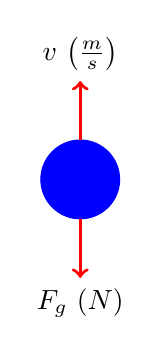
\begin{tikzpicture}
        \draw[blue, fill=blue] (0,0) circle (0.5cm);
        \draw[->, very thick, red] (0, 0.5) -- (0, 1.25) node[above, black] 
        {$v$ $\left( \frac{m}{s} \right)$};
        \draw[->, very thick, red] (0, -0.5) -- (0, -1.25) node[below, black] 
        {$F_g$ $\left( N \right)$};
    \end{tikzpicture}
\end{center}

Intuitively, we know that the ball will slow down (lose kinetic energy) as it 
moves upwards:

$$\Delta KE < 0$$

Since $W = \Delta KE$, we also know that gravity must be doing \textit{negative 
work}. Whenever the direction of the force is opposite the direction of the 
motion, the work done by that force is negative. 
\begin{Exercise}[title=A ball thrown upwards, label=ball_energy]
If the ball has a mass of 0.5 kg, how much kinetic energy does it lose as it moves upwards by 1 m?
\end{Exercise}
\begin{Answer}[ref=ball_energy]
The force acting on the ball is its weight, $F_w = mg$, and we 
will designate this as negative since weight points downwards. Using the 
work-energy theorem, 

$$\Delta KE = F \cdot d = \left( mg \right) \cdot d = \left( 0.5 kg \right) \left(
-9.8 \frac{m}{s^2} \right) \left( 1 m \right) = -4.9 J$$

Therefore, the ball loses 4.9 joules of kinetic energy for every 1 meter it moves 
upwards (the fact it is \textit{losing kinetic energy} is represented by the 
result being negative). Note that this is also the formula for potential energy, so it gained 4.9 J of potential energy.
\end{Answer}

\begin{Exercise}[title = {How far will you slide?}, label = slide]
You are playing softball and have to slide into home. If you sprint at a maximum 
of 10 m/s and the force of friction between you and the ground is 0.3 times your 
weight, how far from the base can you start your slide and still reach home?
\end{Exercise}

\begin{Answer}[ref = slide]
$$F_f \cdot d = \Delta KE = KE_f - KE_i$$

You will reach the maximum distance you can slide when you stop moving, so we will 
use a final velocity of zero, which means a final kinetic energy of zero:
$$F_f \cdot d = -KE_i = \frac{1}{2}mv^2$$

Since the force of friction is 0.3 times your weight, we know that:
$$F_f = 0.3 F_w = 0.3mg$$

Substituting and canceling the mass:
$$\left( 0.3 mg \right) \cdot d = \frac{1}{2}mv^2$$
$$0.3g \cdot d = \frac{1}{2}v^2$$

Since we know g and v, we can solve for d:
$$d = \frac{v^2}{0.6g} = \frac{\left( 10 \frac{m}{s} \right)^2}{0.6 \left( 9.8 
\frac{m}{s^2} \right)} \approx 17 m$$

So you can start your slide as far as 17 m from home.
\end{Answer}

\begin{Exercise}[title = {Ranking Stopping Force}, label = stop]
In drag racing, cars can reach speeds of 150 miles per hour (approximately 240 
kilometers per hour). In order to be able to stop quickly and safely, drag 
racing cars are built with parachutes that deploy at the end of the race. 
Consider a drag race where cars of different masses reach different maximum 
speeds. There is 100 meters between the finish line and the fence surrounding 
the race track. If all the race cars deploy their parachutes at the finish line 
while going their maximum speed, rank the force needed from the parachute to 
stop each car in the required distance from least to greatest:

\begin{center}
	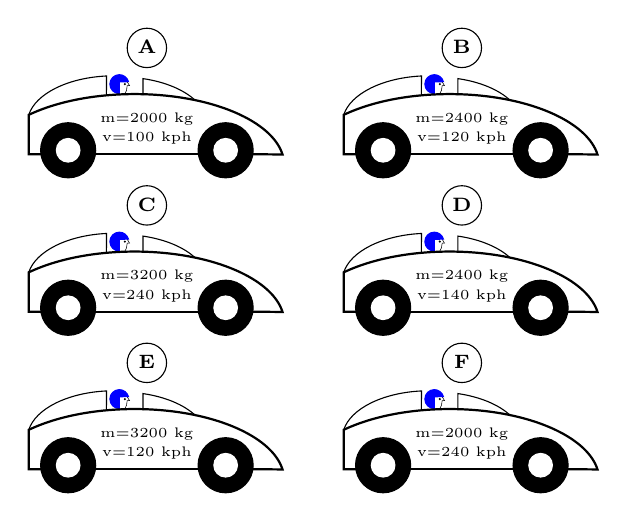
\begin{tikzpicture}
            %CAR A
            %tires
            \draw[black, fill=black] (0.5, 4.35) circle (0.35);
            \draw[white, fill=white] (0.5, 4.35) circle (0.15);
            \draw[black, fill=black] (2.5, 4.35) circle (0.35);
            \draw[white, fill=white] (2.5, 4.35) circle (0.15);

            %driver
            \draw[very thin] (1.25, 5.22) -- (1.28, 5.17) -- (1.25, 5.17) 
            	arc (0:-35:0.2cm and 0.2cm);
            \draw[blue, fill=blue] (1.15, 5.07) arc (270:15:0.12) -- (1.15, 5.22) -- cycle;
            \draw[black, fill=black] (1.22, 5.19) circle (0.05mm);
            
            %outline
            \draw[black, thick] (0.8, 4.3) -- (2.2, 4.3);
            \draw[black, thick] (0.2, 4.3) -- (0, 4.3) -- (0, 4.8) 
            	arc (135:8.5:1.9cm and 0.9cm) -- (2.8, 4.3);
            \draw[black] (0, 4.8) arc (170:95:1.1cm and 0.6cm) -- (.986, 5.05); 
            \draw[black] (1.45, 5.05) -- (1.45, 5.26) arc (75:30:1.1cm and 0.6cm); 

            %speed and mass info
            \node[font=\tiny] at (1.5, 4.75) {m=2000 kg};
            \node[font=\tiny] at (1.5, 4.5) {v=100 kph};

            %car label
            \draw[black] (1.5, 5.65) circle (0.25) 
            	node[above, font = \scriptsize, yshift = -0.2cm] {\textbf{A}};

            %CAR B
            %tires
            \draw[black, fill=black] (4.5, 4.35) circle (0.35);
            \draw[white, fill=white] (4.5, 4.35) circle (0.15);
            \draw[black, fill=black] (6.5, 4.35) circle (0.35);
            \draw[white, fill=white] (6.5, 4.35) circle (0.15);

            %driver
            \draw[very thin] (5.25, 5.22) -- (5.28, 5.17) -- (5.25, 5.17) 
            	arc (0:-35:0.2cm and 0.2cm);
            \draw[blue, fill=blue] (5.15, 5.07) arc (270:15:0.12) -- (5.15, 5.22) -- cycle;
            \draw[black, fill=black] (5.22, 5.19) circle (0.05mm);
            
            %outline
            \draw[black, thick] (4.8, 4.3) -- (6.2, 4.3);
            \draw[black, thick] (4.2, 4.3) -- (4, 4.3) -- (4, 4.8) 
            	arc (135:8.5:1.9cm and 0.9cm) -- (6.8, 4.3);
            \draw[black] (4, 4.8) arc (170:95:1.1cm and 0.6cm) -- (4.986, 5.05); 
            \draw[black] (5.45, 5.05) -- (5.45, 5.26) arc (75:30:1.1cm and 0.6cm); 

            %speed and mass info
            \node[font=\tiny] at (5.5, 4.75) {m=2400 kg};
            \node[font=\tiny] at (5.5, 4.5) {v=120 kph};

            %car label
            \draw[black] (5.5, 5.65) circle (0.25) 
            	node[above, font = \scriptsize, yshift = -0.2cm] {\textbf{B}};
            
            %CAR C
            %tires
            \draw[black, fill=black] (0.5, 2.35) circle (0.35);
            \draw[white, fill=white] (0.5, 2.35) circle (0.15);
            \draw[black, fill=black] (2.5, 2.35) circle (0.35);
            \draw[white, fill=white] (2.5, 2.35) circle (0.15);

            %driver
            \draw[very thin] (1.25, 3.22) -- (1.28, 3.17) -- (1.25, 3.17) 
            	arc (0:-35:0.2cm and 0.2cm);
            \draw[blue, fill=blue] (1.15, 3.07) arc (270:15:0.12) -- (1.15, 3.22) -- cycle;
            \draw[black, fill=black] (1.22, 3.19) circle (0.05mm);
            
            %outline
            \draw[black, thick] (0.8, 2.3) -- (2.2, 2.3);
            \draw[black, thick] (0.2, 2.3) -- (0, 2.3) -- (0, 2.8) 
            	arc (135:8.5:1.9cm and 0.9cm) -- (2.8, 2.3);
            \draw[black] (0, 2.8) arc (170:95:1.1cm and 0.6cm) -- (.986, 3.05); 
            \draw[black] (1.45, 3.05) -- (1.45, 3.26) arc (75:30:1.1cm and 0.6cm); 

            %speed and mass info
            \node[font=\tiny] at (1.5, 2.75) {m=3200 kg};
            \node[font=\tiny] at (1.5, 2.5) {v=240 kph};

            %car label
            \draw[black] (1.5, 3.65) circle (0.25) 
            	node[above, font = \scriptsize, yshift = -0.2cm] {\textbf{C}};

            %CAR D
            %tires
            \draw[black, fill=black] (4.5, 2.35) circle (0.35);
            \draw[white, fill=white] (4.5, 2.35) circle (0.15);
            \draw[black, fill=black] (6.5, 2.35) circle (0.35);
            \draw[white, fill=white] (6.5, 2.35) circle (0.15);

            %driver
            \draw[very thin] (5.25, 3.22) -- (5.28, 3.17) -- (5.25, 3.17) 
            	arc (0:-35:0.2cm and 0.2cm);
            \draw[blue, fill=blue] (5.15, 3.07) arc (270:15:0.12) -- (5.15, 3.22) -- cycle;
            \draw[black, fill=black] (5.22, 3.19) circle (0.05mm);
            
            %outline
            \draw[black, thick] (4.8, 2.3) -- (6.2, 2.3);
            \draw[black, thick] (4.2, 2.3) -- (4, 2.3) -- (4, 2.8) 
            	arc (135:8.5:1.9cm and 0.9cm) -- (6.8, 2.3);
            \draw[black] (4, 2.8) arc (170:95:1.1cm and 0.6cm) -- (4.986, 3.05); 
            \draw[black] (5.45, 3.05) -- (5.45, 3.26) arc (75:30:1.1cm and 0.6cm); 

            %speed and mass info
            \node[font=\tiny] at (5.5, 2.75) {m=2400 kg};
            \node[font=\tiny] at (5.5, 2.5) {v=140 kph};

            %car label
            \draw[black] (5.5, 3.65) circle (0.25) 
            	node[above, font = \scriptsize, yshift = -0.2cm] {\textbf{D}};
            
            %CAR E
            %tires
            \draw[black, fill=black] (0.5, 0.35) circle (0.35);
            \draw[white, fill=white] (0.5, 0.35) circle (0.15);
            \draw[black, fill=black] (2.5, 0.35) circle (0.35);
            \draw[white, fill=white] (2.5, 0.35) circle (0.15);

            %driver
            \draw[very thin] (1.25, 1.22) -- (1.28, 1.17) -- (1.25, 1.17) 
            	arc (0:-35:0.2cm and 0.2cm);
            \draw[blue, fill=blue] (1.15, 1.07) arc (270:15:0.12) -- (1.15, 1.22) -- cycle;
            \draw[black, fill=black] (1.22, 1.19) circle (0.05mm);
            
            %outline
            \draw[black, thick] (0.8, 0.3) -- (2.2, 0.3);
            \draw[black, thick] (0.2, 0.3) -- (0, 0.3) -- (0, 0.8) 
            	arc (135:8.5:1.9cm and 0.9cm) -- (2.8, 0.3);
            \draw[black] (0, 0.8) arc (170:95:1.1cm and 0.6cm) -- (.986, 1.05); 
            \draw[black] (1.45, 1.05) -- (1.45, 1.26) arc (75:30:1.1cm and 0.6cm); 

            %speed and mass info
            \node[font=\tiny] at (1.5, 0.75) {m=3200 kg};
            \node[font=\tiny] at (1.5, 0.5) {v=120 kph};

            %car label
            \draw[black] (1.5, 1.65) circle (0.25) 
            	node[above, font = \scriptsize, yshift = -0.2cm] {\textbf{E}};

            %CAR F
            %tires
            \draw[black, fill=black] (4.5, 0.35) circle (0.35);
            \draw[white, fill=white] (4.5, 0.35) circle (0.15);
            \draw[black, fill=black] (6.5, 0.35) circle (0.35);
            \draw[white, fill=white] (6.5, 0.35) circle (0.15);

            %driver
            \draw[very thin] (5.25, 1.22) -- (5.28, 1.17) -- (5.25, 1.17) 
            	arc (0:-35:0.2cm and 0.2cm);
            \draw[blue, fill=blue] (5.15, 1.07) arc (270:15:0.12) -- (5.15, 1.22) -- cycle;
            \draw[black, fill=black] (5.22, 1.19) circle (0.05mm);
            
            %outline
            \draw[black, thick] (4.8, 0.3) -- (6.2, 0.3);
            \draw[black, thick] (4.2, 0.3) -- (4, 0.3) -- (4, 0.8) 
            	arc (135:8.5:1.9cm and 0.9cm) -- (6.8, 0.3);
            \draw[black] (4, 0.8) arc (170:95:1.1cm and 0.6cm) -- (4.986, 1.05); 
            \draw[black] (5.45, 1.05) -- (5.45, 1.26) arc (75:30:1.1cm and 0.6cm); 

            %speed and mass info
            \node[font=\tiny] at (5.5, 0.75) {m=2000 kg};
            \node[font=\tiny] at (5.5, 0.5) {v=240 kph};

            %car label
            \draw[black] (5.5, 1.65) circle (0.25) 
            	node[above, font = \scriptsize, yshift = -0.2cm] {\textbf{F}};
	\end{tikzpicture}
\end{center}
\end{Exercise}

\begin{Answer}[ref = stop]
Since all the cars need to stop in the same distance, the cars with the 
greatest kinetic energy will take the most force to stop. Calculating the 
kinetic energies (we will not change the units from kilometers per hour to meters 
per second, since we are just comparing the values):

\begin{center}
	\begin{tabular}{|c|c|c|c|}\hline
	Car & Mass [kg] & Max speed [kph] & KE [kg $(kph)^2$]\\\hline
	A & 2000 & 100 & $1 \times 10^7$\\\hline
	B & 2400 & 120 & $1.728 \times 10^7$\\\hline
	C & 3200 & 240 & $9.216 \times 10^7$\\\hline
	D & 2400 & 140 & $2.352 \times 10^7$\\\hline
	E & 3200 & 120 & $2.304 \times 10^7$\\\hline
	F & 2000 & 240 & $5.76 \times 10^7$\\\hline
	\end{tabular}
\end{center}

The correct ranking is A, B, E, D, F, C. 
\end{Answer}

\subsection{Forces that do no work}
If the object you are pushing does not move, or the applied force is perpendicular 
to the direction of motion, that force does no work. Let us look at a few examples:

\subsection{Pushing Against an Immobile Object}
At the beginning of the chapter, we said that when you push on a wall, you do not 
do any work. Why is this? Well, if the wall is a good wall (that is, strong 
enough to not be pushed over by a person), the wall will not move while you push on 
it. This means the distance over which your push is applied is zero, and 
therefore the work done ($F \cdot d = F \cdot 0 = 0$) is zero joules.

\subsection{Walking Across a Room with a Book}
Imagine holding a book flat on your hands and walking at a constant velocity. 
Your hand is applying an upwards force to the book, but the book is moving 
horizontally. This means the force and direction of motion are 
\textit{perpendicular}. Recall from the beginning of the chapter that if the 
force and distance are not parallel, then the work is given by $W = F \cdot d 
\cos{\left( \theta \right)}$. (When the vectors are parallel, $\theta = 0$ and 
$\cos{\left( \theta \right)} = 1$, while when the vectors point in opposite 
directions, $\theta = 180^{\circ}$ and $\cos{ \left( \theta \right)} = -1$.) 
When the vectors are perpendicular, then $\theta = 90^{\circ}$ and $\cos{ \left( 
\theta \right)} = 0$. Therefore, $W = 0$ as well and the upward force of your 
hands does no net work. 

\subsection{Circular Motion}
We will discuss circular motion further in a subsequent chapter. For now, know 
that constant-speed circular motion is caused by a constant-magnitude force that 
always points to the center of the circle the object is moving in. For example, 
you can take a weight on the end of a string and spin it. The tension in the 
string spins the weight, and the string always points from the object to your 
hand (the center of the weight's circular path). For a satellite, that force is 
gravitational attraction to the Earth.

\begin{center}
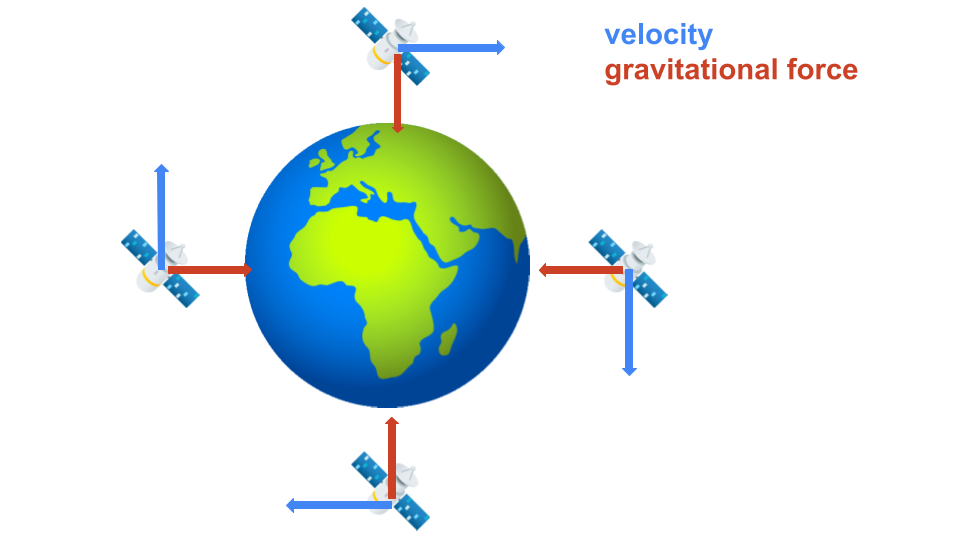
\includegraphics[width=4in]{satellite.png}
\end{center}

As a result, the force changes the \textit{direction}, but not the 
\textit{magnitude} of the satellite's velocity. Let us re-examine the equation 
for kinetic energy:

$$KE = \frac{1}{2}mv^2$$

Since the velocity is squared, the direction of motion does not affect the kinetic 
energy (a ball moving at 5 m/s upwards has the same kinetic energy as if the ball 
were moving at 5 m/s downwards). So, a force that causes circular motion does not 
change a circling object's kinetic energy, and therefore does no work (as 
expected when force and direction of motion are perpendicular)!

\section{Efficiency and Power}
Energy is never destroyed, but it does leak away into forms we cannot use, usually heat. Efficiency measures how much of the energy you put in does the job you wanted.\index{efficiency}

In terms of an equation, efficiency is the ratio of the useful energy output to 
the total energy input. It is usually expressed as a percentage.
\begin{mdframed}[style=important, frametitle={Formula for Efficiency}]
\[
\text{Efficiency} = \frac{\text{Useful Energy Output}}{\text{Total Energy Input}} 
\times 100\%
\]
\end{mdframed}
where the useful energy output is the energy that is actually used to do work or 
complete a task, and the total energy input is the total energy consumed by the 
system.

A machine is considered 100\% efficient only if all the input work is converted 
into useful output work, with no energy lost to heat, friction, or sound. 100\% 
efficient processes do not exist in real life: every process loses some useful 
energy to heat. 

For example, when a car engine consumes the chemical energy in gasoline, only
about 20\% of the energy consumed is used to turn the wheels. Most of the energy 
is actually lost as heat. If you run a car for a while, the engine gets very hot, 
as does the exhaust coming from the tailpipe.

A human is about 25\% efficient. Most of the loss is in the heat produced during 
the chemical reactions that turns food into motion.
% ADD: Cellular Respiration

So if you want to make a machine more efficient, follow the heat. Wherever it gets hot, energy is leaking away.

Light bulbs are an interesting case. To get the same amount of light of a 60 watt 
incandescent bulb, you can use an 8 watt LED or a 16 watt fluorescent light. This 
is why we say that the LED light is much more efficient. If you run both, the 
incandescent bulb will consume 1.44 kilowatt-hours; the LED will consume only 
0.192 kilowatt-hours. 

In addition to light, the incandescent bulb is producing a lot of heat. If it
is inside your house, what happens to the heat? It warms your house.

In the winter, when you want light and heat, the incandescent bulb is
100\% efficient!

Of course, this also means the reverse is true. In the summer, if you are running 
the air conditioner to cool down your house, the incandescent bulb is worse than 
just ``inefficient at making light'' --- it is actually counteracting the air 
conditioner!

\begin{Exercise}[title=Unit Costs, label=efficiency1]
A machine is rated to produce 500 bolts per hour, but in actual operation it runs at only $82\%$ efficiency due to loss and scraps.
The machine requires \mathdollar 24 of electricity per hour to run.
\begin{enumerate}[label=(\alph*)]
  \item What is the actual output of bolts per hour?
  \item What is the unit cost (cost per bolt) of the production?
\end{enumerate}

\end{Exercise}
\begin{Answer}[ref=efficiency1]
  \begin{enumerate}[label=(\alph*)]
    \item $500 \times 0.82 = 410 \text{ bolts}$
    \item $\frac{\mathdollar24}{410} \approx \mathdollar 0.06$
  \end{enumerate}
\end{Answer}

\emph{Power}\index{power} is how fast work gets done. Suppose we each carry the same box up the stairs, doing 1000 J of work. I take 10 minutes; you take 5. We did the same work, but you did it twice as fast, so you were twice as \emph{powerful}.

\begin{mdframed}[style=important, frametitle={Formula for Power}]
	\[\text{Power} = \frac{\text{Work}}{\text{Time}} \implies P = \frac{W}{t}\]
  Power is represented by the unit \index{watt}watt ($\text{W}$), defined as one joule per second ($\text{J/s}$).
	Since power is a rate, we can also express it using calculus:
	\[P=\frac{dW}{dt}\]

	For a constant force moving an object at speed $v$ in the direction of the force, $P=\frac{F d}{t} = F v$, since $v = \frac{d}{t}$.
\end{mdframed}

%CONSTANT FORCE
\begin{Exercise}[title=Hydraulic Piston Problem,label=power1]
A hydraulic piston pushes a crate horizontally across the floor with a constant force of 450 N.
During operation, the piston moves the crate 1.8 meters in 0.75 seconds.

\begin{enumerate}[label=(\alph*)]
  \item How much work does the piston do on the crate?
  \item What is the power output of the piston during this motion?
\end{enumerate}
\end{Exercise}
\begin{Answer}[ref=power1]
\begin{enumerate}[label=(\alph*)]
  \item $$W = F\cdot d = 450 \cdot  1.8 =810 \text{ J}$$
  \item $$P = \frac{W}{t} = \frac{810}{.75} = 1080 \text{ W}$$
  Alternatively,
  $$v = \frac{d}{t} = \frac{1.8}{0.75} = 2.4\ \text{m/s}$$
  $$P = F\cdot v = 450 \cdot 2.4 = 1080 \text{ W}$$
\end{enumerate}
\end{Answer}

%VARIABLE FORCE
\begin{Exercise}[title=Spring Power, label=power2]
A compressed spring launches a small block. The spring delivers $120$ W of power while releasing its stored energy over $0.40$ seconds. The spring constant is $k = 800$ N/m.

How far was the spring compressed?
\end{Exercise}

\begin{Answer}[ref=power2]
\begin{align*}
  P &= \frac{E}{t} \\
  E &= P\cdot t = 120 (0.4) = 48 \text{ J}
\end{align*}
So 48 J of energy is stored into the spring. We can find the spring's PE converted to distance by:
\begin{align*}
  E &= \frac{1}{2}kx^2\\
  48 &= \frac{1}{2}(800)x^2 \\
  x^2 &= \frac{48}{400} \\ 
  x &= \sqrt{0.12} \approx 0.346 \text{ m}
\end{align*}
So the spring had to have been compressed 34.6 cm.
\end{Answer}

\begin{Exercise}[title=Elevator Lift, label = elevatorPE]
An elevator motor lifts a $750 \text{ kg}$ cabin vertically upward a distance of $18 \text{ m}$ in $12 \text{ s}$. The motor consumes electrical energy at a rate of 
$18 \text{ kW}$. 

\begin{enumerate}[label=(\alph*)]
  \item Compute the total electrical energy consumed during the lift. Note that $1 \text{ kW} = 1000 \text{ watts} = 1000 \text{ J/s}$
  \item Determine the gravitational potential energy gained by the elevator.
  \item Calculate the efficiency of the motor during this lift.
\end{enumerate}

\end{Exercise}
\begin{Answer}[ref=elevatorPE]
  
\begin{enumerate}[label=(\alph*)]
  \item Electrical energy input can be calculated as $E= Pt = 18 \text{ kW} \times 1000 \text{ J/s} \times 12 \text{ sec} = 216,000 \text{ J}$. 
  \item The elevator travels $18 \text{ m}$ upwards, so the total gravitational potential energy is $mgh = 750(9.8)(18) = 132,300 \text{ J}$. 
  \item The efficiency can be calculated as $\frac{\text{Useful Output}}{\text{Total Input}} = \frac{132,300}{216,000} \approx 61.3\%$
\end{enumerate}
\end{Answer}
